\documentclass[11pt]{article}
\usepackage[margin=1in]{geometry}
\usepackage{booktabs}
\usepackage{array}
\usepackage{graphicx}
\usepackage{enumitem}
\usepackage[htt]{hyphenat}
\sloppy
\usepackage[colorlinks=true,urlcolor=blue,linkcolor=black]{hyperref}

\title{Wearables and Habits: Staggered DiD, Placebos and Shoe Bundling\\\large Issue \#7}
\date{4 October 2026}
\author{}

\begin{document}
\maketitle

\section{Summary}
Exploratory staggered DiD (Callaway--Sant'Anna, never-treated controls, no covariates, user-quarter panel, outcome = any purchase in the quarter) of first wearable purchase on running-related and other purchases. All event studies use the universal base period, so the \textbf{reference period is $t=-1$} (not $t=0$); the coefficient at $-1$ is zero by construction.
\begin{itemize}[nosep]
\item \textbf{Pre-trends are strong, so the reduced form is not credible as is.} Treated users purchase \emph{less} than controls 2--8 quarters before adoption, relative to $t=-1$, in almost every outcome (Figure~\ref{fig:main}), including the placebos (Figure~\ref{fig:plac}). Treated users' purchasing is ramping up into adoption (consistent with the rising pre-adoption purchasing noted in \#5).
\item \textbf{No detectable post-adoption increase in running purchases.} Post ATT (quarters 1--8) for running shoes is $-0.016$ (0.009), running-related $-0.033$ (0.016), fitness gear $-0.020$ (0.014), supplements $+0.022$ (0.017), medication $-0.005$ (0.014). Negative post estimates relative to $t=-1$ mostly reflect the $t=-1$ peak in a ramp-up, not a causal drop.
\item \textbf{Placebos mostly small, but the general-intensity outcomes are not.} Pet, books, gift cards, cables, cleaning, grocery and (conditional) shoe price are all within about 2 SE of zero post, yet show the same pre-trend as the main outcomes. Total purchases $\ln(1+n)$ and spend fall post ($-0.11$, $-0.20$) after a pronounced run-up ($t=0$ spike of $+0.20$ in $\ln(1+n)$ from the device order itself).
\item \textbf{Bundling is thin.} Only 30 of the 570 adopters buy a running shoe within $\pm1$ month of the device (24 of 447 clean). Excluding the bundled shoe, no outcome differs significantly between bundlers and non-bundlers except fitness gear (difference $-0.144$, SE 0.072, borderline), and the bundler estimates are very imprecise.
\item \textbf{Running shoes as the treatment:} buying running shoes does not predict a later wearable purchase ($+0.001$, SE 0.007), but does predict later non-shoe running-related purchases ($+0.029$, SE 0.014; $+0.041$ among users who never buy a wearable), with the caveat of pre-trends. Repeat shoe purchase is $+0.082$ (mechanical replacement).
\end{itemize}

\section{Design}
\begin{itemize}[nosep]
\item \textbf{Panel:} user-quarter over each user's observed window, truncated at 2023-03 (usable window from \#5); zeros filled; unbalanced panel. Built by \texttt{code/scripts/prep\_design\_panel.py}; estimated by \texttt{code/scripts/design\_did.R}; figures/tables by \texttt{design\_did\_figs.py}.
\item \textbf{Treated:} first non-kids wearable (Category \texttt{WEARABLE\_COMPUTER}/\texttt{BIOMETRIC\_MONITOR}) with $\geq$12 months pre and post (570 users); ``clean'' variant (447 users) also requires price $\geq$\$40, quantity 1, not an accessory; non-clean adopters are dropped from the clean sample. \textbf{Controls:} users who never buy a wearable (about 4{,}100). Adopters with $<$12m pre/post are dropped.
\item \textbf{Estimator:} \texttt{did::att\_gt}, \texttt{est\_method="reg"}, no covariates, universal base period, analytic SEs clustered by user, event window $-8$ to $+8$ quarters. ``Post ATT'' is the average of $e=1,\dots,8$ (excludes $e=0$, which contains the device purchase itself).
\item \textbf{Outcomes:} indicators for any purchase in the quarter: running shoe, running-related keyword, fitness gear, supplements, medication (definitions from \#5). \textbf{Placebos:} pet, books, gift cards, cables/chargers/batteries, cleaning agents, grocery/food; $\ln$ average price of shoes (SHOES category, only quarters with a shoe purchase); and general intensity $\ln(1+n)$ and $\ln(1+\mathrm{spend})$.
\item \textbf{Bundling:} bundler = a running shoe bought within $\pm1$ month of the first wearable. For adopters the bundled shoe is removed from the shoe and running-related outcomes.
\item \textbf{Shoe as treatment:} first running shoe (604 users with $\geq$12m pre and post) vs.\ never-running-shoe users, outcomes wearable, non-shoe running-related, fitness gear, supplements, repeat shoe, with a version dropping all wearable adopters.
\end{itemize}

\section{Main outcomes and placebos}
\begin{center}\small\begin{tabular}{lrrr}
\toprule
Outcome & Post ATT (SE) & Pre-test p & N treated \\
\midrule
Running shoe & -0.016 (0.009) & n/a & 570 \\
Running-related (keyword) & -0.033 (0.016) & 0.000 & 570 \\
Fitness gear & -0.020 (0.014) & 0.000 & 570 \\
Supplements & 0.022 (0.017) & 0.000 & 570 \\
Medication & -0.005 (0.014) & 0.000 & 570 \\
PLACEBO: pet & -0.024 (0.016) & 0.000 & 570 \\
PLACEBO: books & -0.001 (0.019) & 0.000 & 570 \\
PLACEBO: gift cards & 0.002 (0.014) & 0.000 & 570 \\
PLACEBO: cables/batteries & 0.004 (0.019) & 0.000 & 570 \\
PLACEBO: cleaning & 0.021 (0.014) & 0.000 & 570 \\
PLACEBO: grocery/food & 0.020 (0.015) & 0.000 & 570 \\
PLACEBO: ln shoe price (cond.) & -0.046 (0.068) & 0.000 & 441 \\
General: ln(1+\#purchases) & -0.110 (0.034) & 0.000 & 570 \\
General: ln(1+spend) & -0.203 (0.053) & 0.000 & 570 \\
\bottomrule
\end{tabular}
\end{center}
The pre-test column is the joint Wald test of the pre-period ATTs from \texttt{did}; it is $0.000$ almost everywhere and n/a when the covariance matrix is singular, so rely on the plots. The clean-sample estimates are similar (Table in \texttt{design\_tab\_main\_clean.tex}; running-related $-0.027$ (0.018), shoe $-0.011$ (0.011)).
\begin{figure}[h]\centering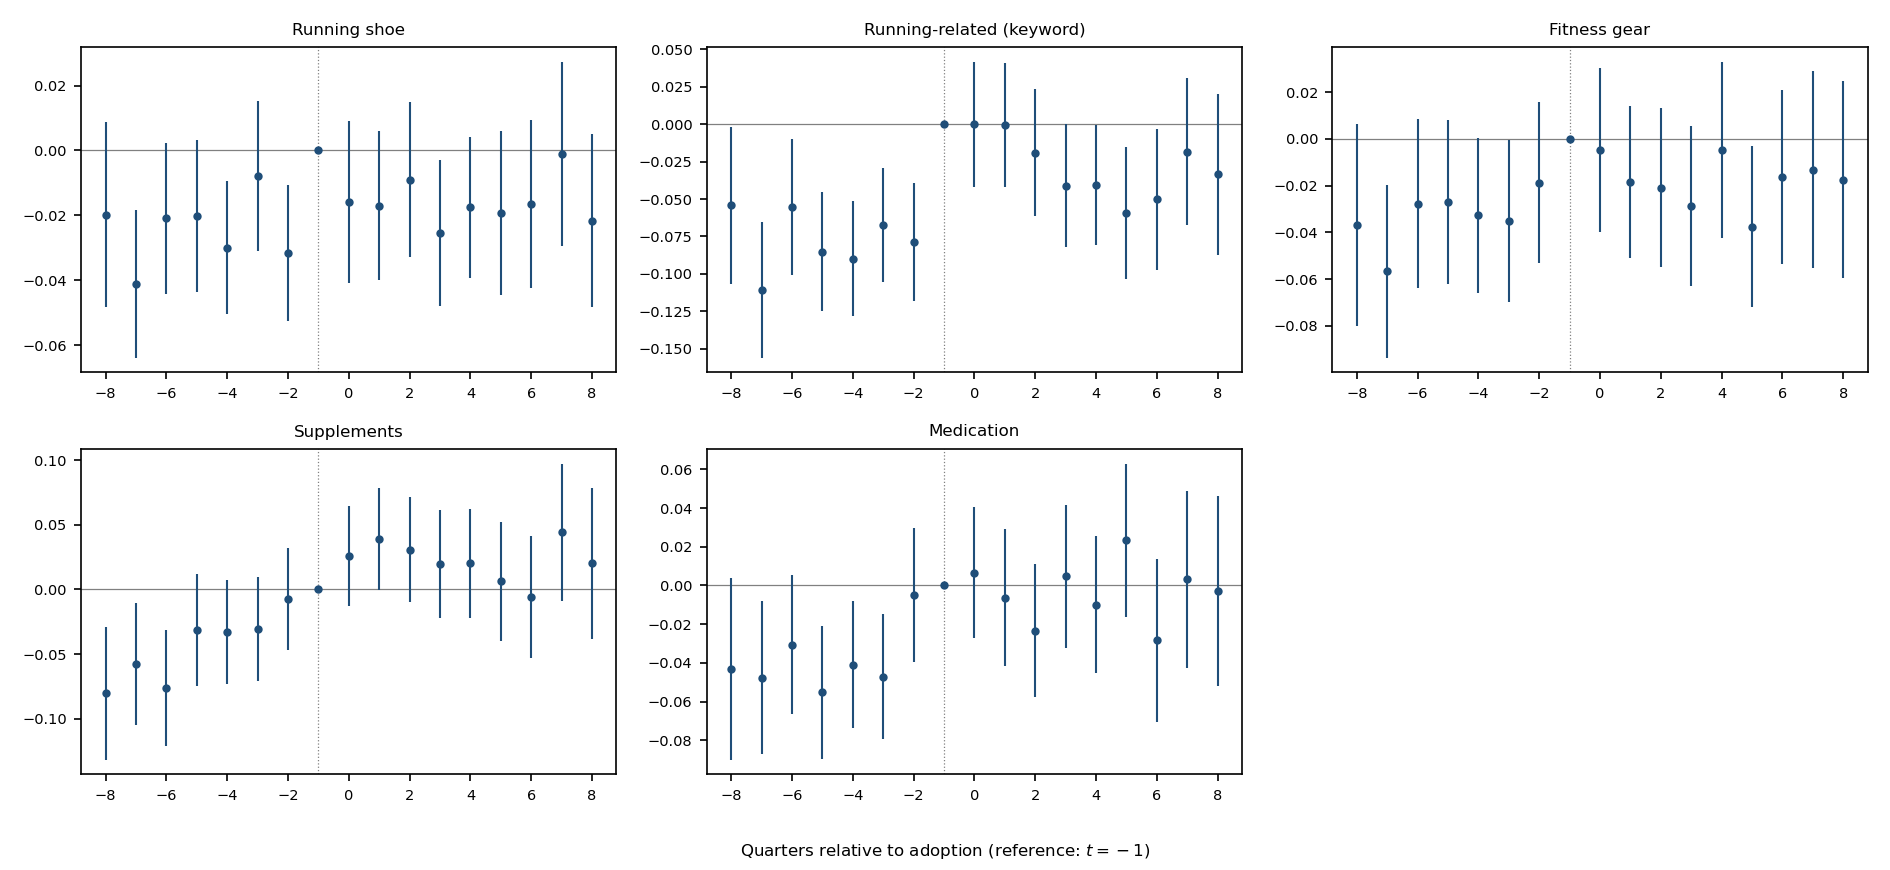
\includegraphics[width=\textwidth]{../code/analysis/outputs/design_es_main.png}
\caption{Event studies, main outcomes (570 adopters). 95\% CIs; reference $t=-1$.}\label{fig:main}\end{figure}
\begin{figure}[h]\centering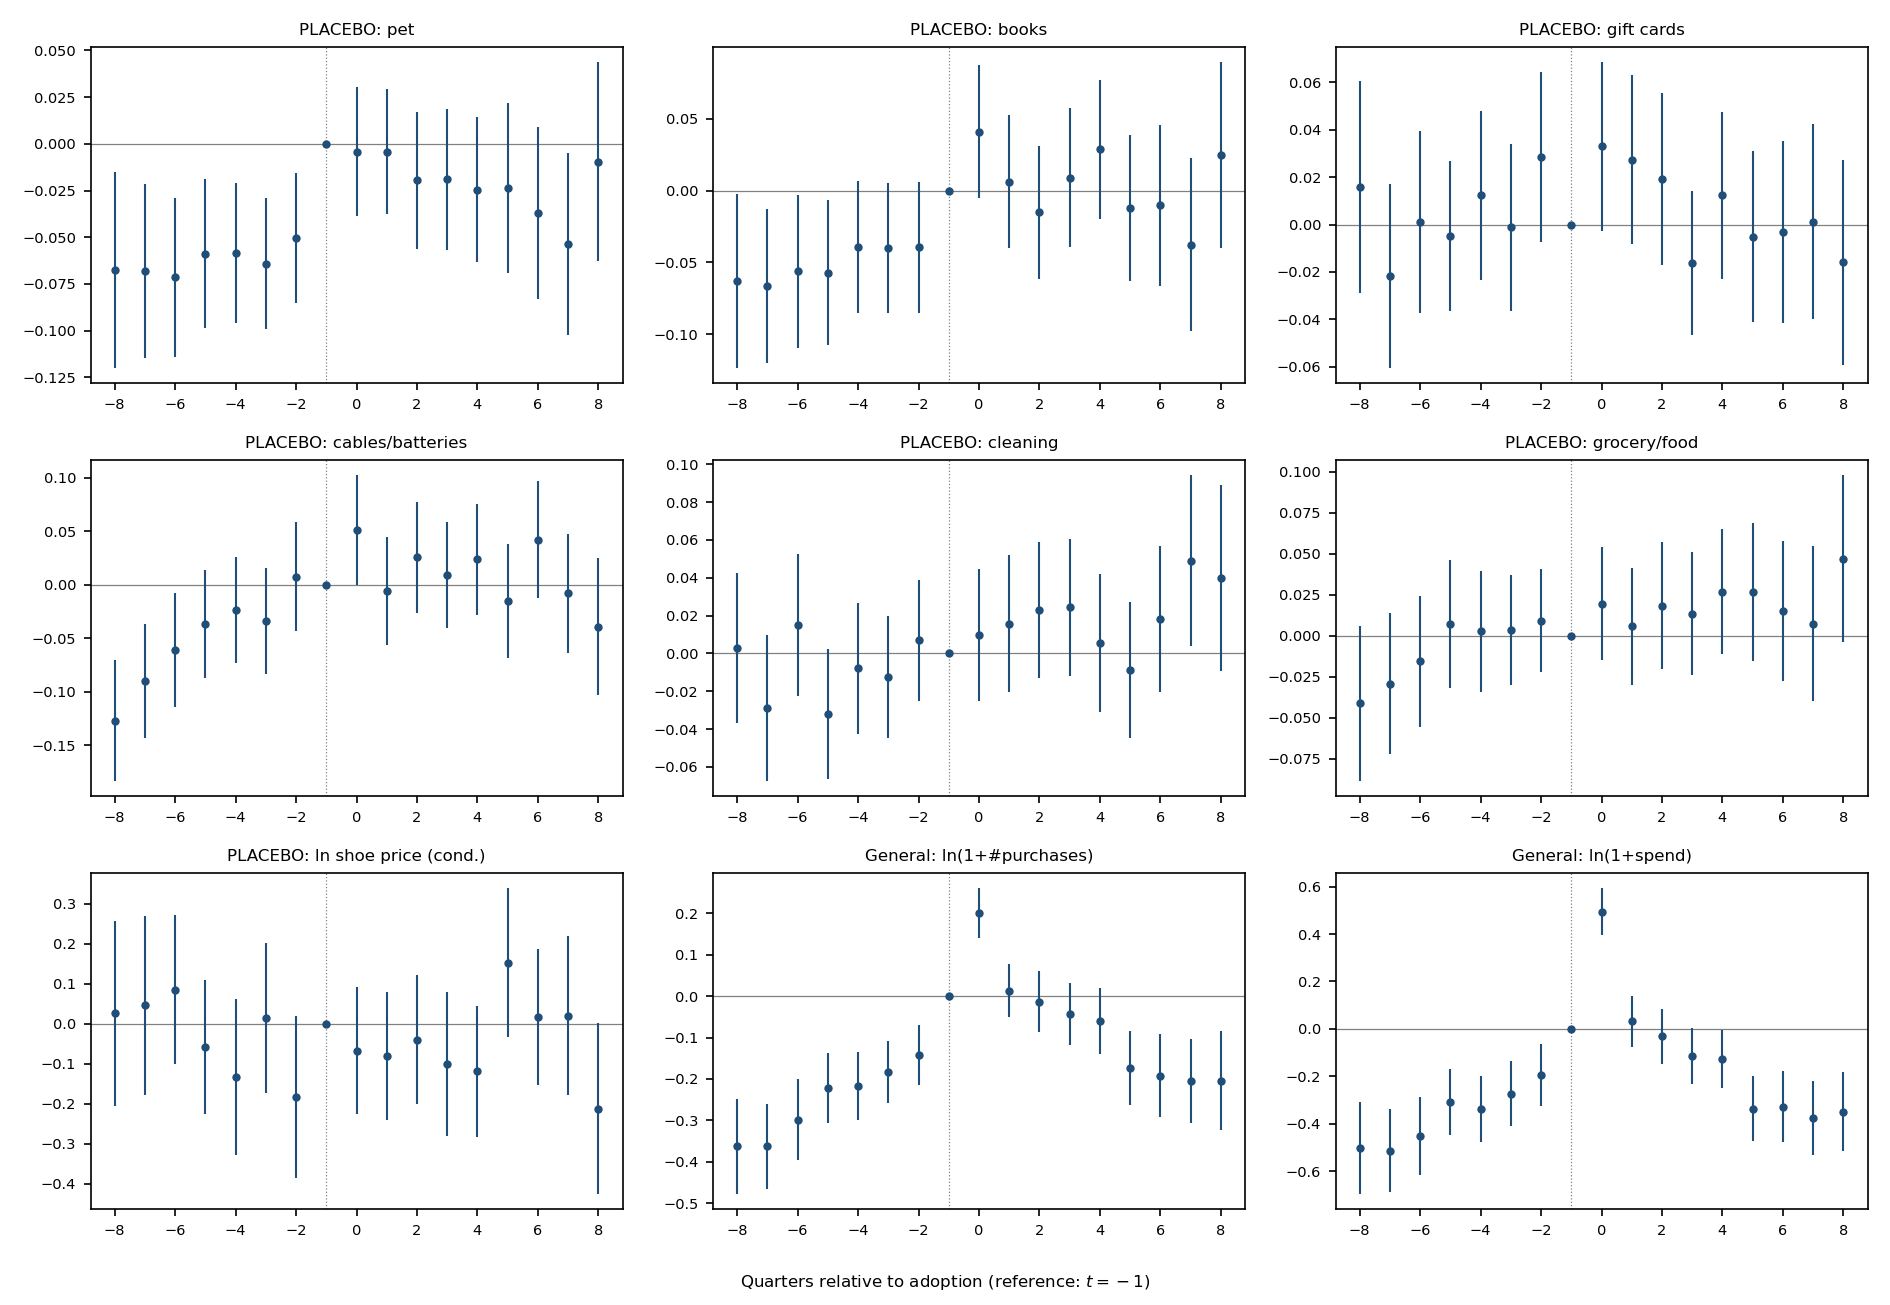
\includegraphics[width=\textwidth]{../code/analysis/outputs/design_es_placebo.png}
\caption{Event studies, placebo and general-intensity outcomes. Placebos show the same pre-trend as the main outcomes.}\label{fig:plac}\end{figure}

\section{Running-shoe bundling}
\begin{center}\small\begin{tabular}{lrrr}
\toprule
Outcome & Bundlers (N=30) & Non-bundlers (N=540) & Difference \\
\midrule
Fitness gear & -0.156 (0.071) & -0.012 (0.014) & -0.144 (0.072) \\
Running-related (ex-bundle) & -0.113 (0.083) & -0.016 (0.016) & -0.098 (0.084) \\
Running shoe (ex-bundle) & -0.005 (0.053) & -0.014 (0.009) & 0.008 (0.054) \\
Supplements & -0.028 (0.073) & 0.024 (0.017) & -0.052 (0.075) \\
\bottomrule
\end{tabular}
\end{center}
Post ATT (SE); the difference SE assumes independence (shared controls make it slightly conservative or not, unchecked). Pre-test for bundlers is not available (30 users).
\begin{figure}[h]\centering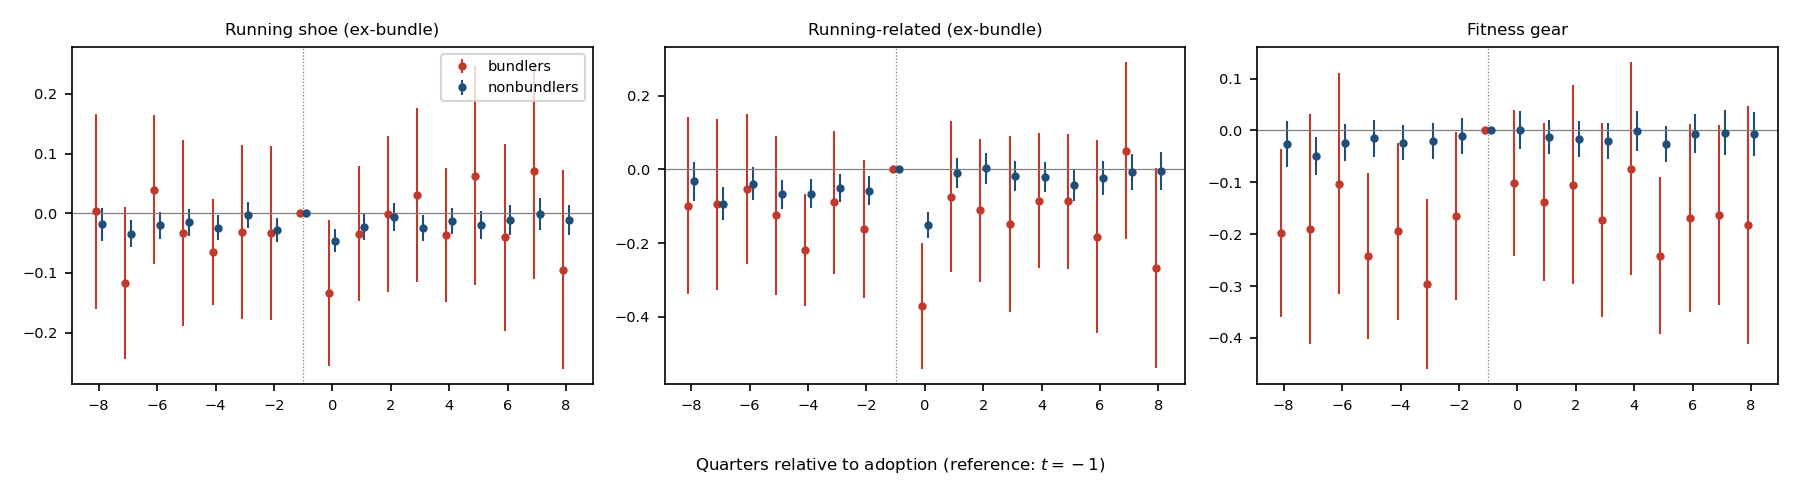
\includegraphics[width=\textwidth]{../code/analysis/outputs/design_es_bundle.png}
\caption{Bundlers (red, 30) vs non-bundlers (blue, 540), bundled shoe excluded from outcomes.}\label{fig:bundle}\end{figure}

\section{Running shoes as the treatment}
\begin{center}\small\begin{tabular}{lrrr}
\toprule
Outcome & Post ATT (SE) & Pre-test p & N treated \\
\midrule
Wearable purchase & 0.001 (0.007) & n/a & 604 \\
Running-related, non-shoe & 0.029 (0.014) & n/a & 604 \\
Fitness gear & 0.001 (0.013) & 0.000 & 604 \\
Supplements & -0.003 (0.017) & 0.000 & 604 \\
Running shoe (repeat) & 0.082 (0.005) & n/a & 604 \\
PLACEBO-ish: medication & -0.002 (0.013) & n/a & 604 \\
PLACEBO: pet & -0.019 (0.017) & 0.000 & 604 \\
PLACEBO: books & -0.035 (0.018) & 0.000 & 604 \\
\bottomrule
\end{tabular}
\end{center}
\begin{figure}[h]\centering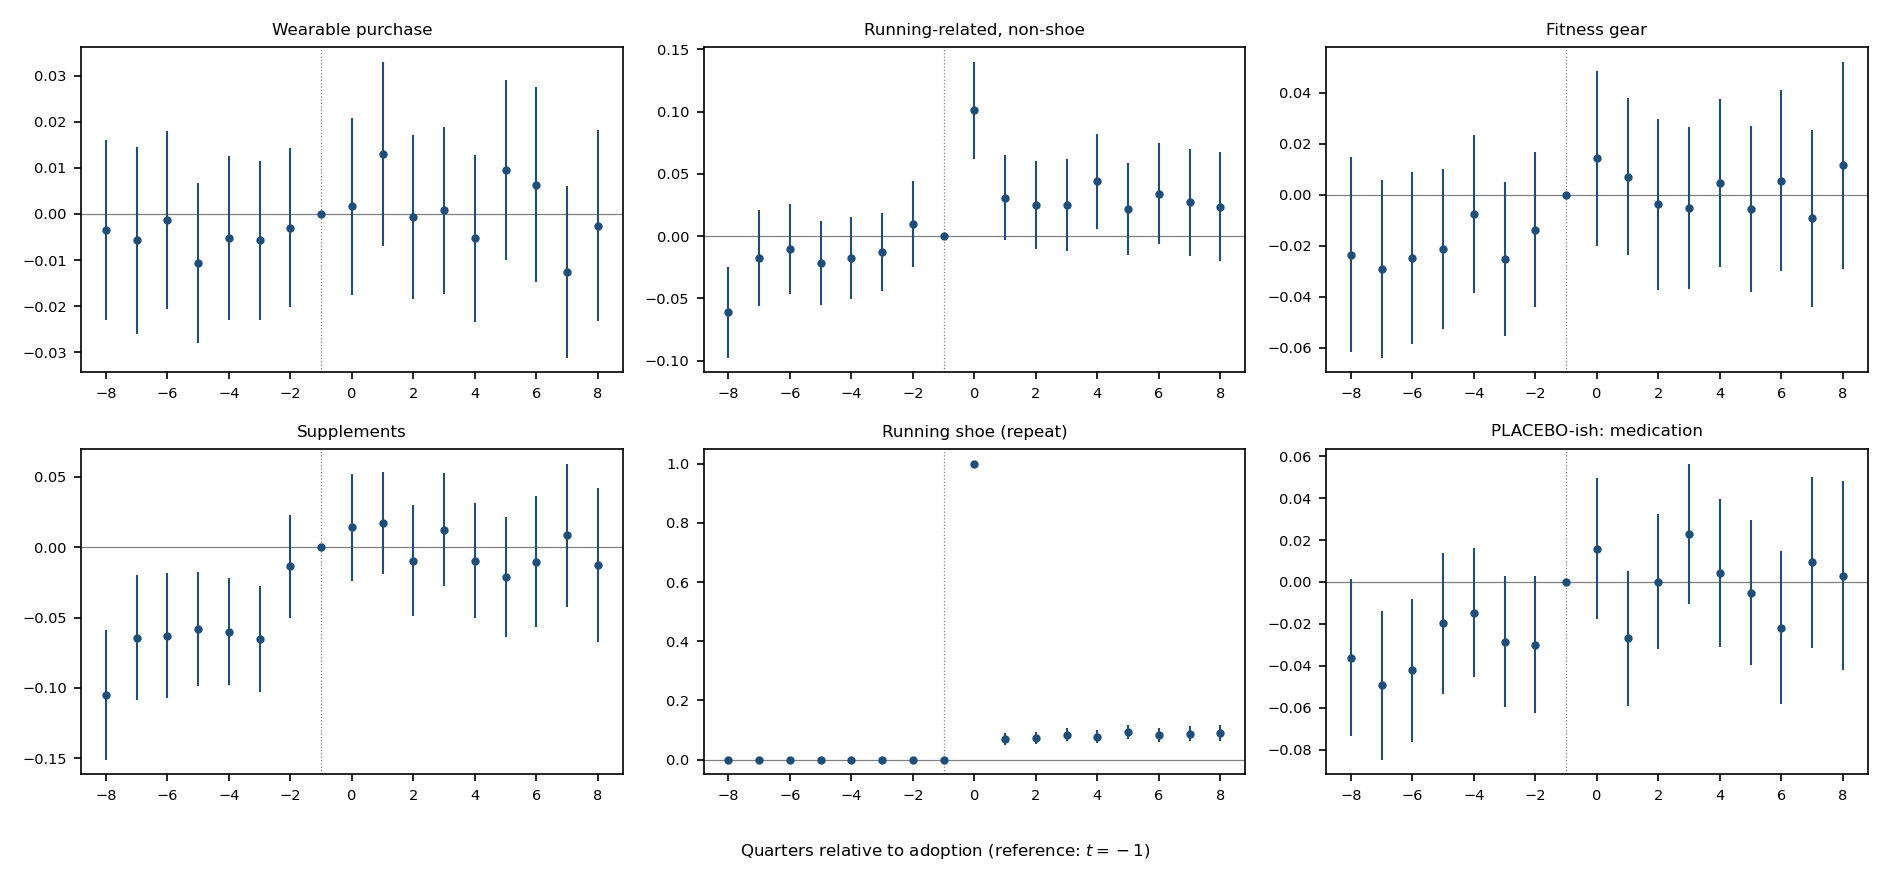
\includegraphics[width=\textwidth]{../code/analysis/outputs/design_es_shoe_treat.png}
\caption{Event studies with the first running-shoe purchase as treatment.}\label{fig:shoe}\end{figure}
Dropping wearable adopters (399 treated): non-shoe running-related $+0.041$ (0.015), repeat shoe $+0.074$ (0.006); the wearable outcome is undefined there by construction.

\section{Pitfalls and follow-ups}
\begin{itemize}[nosep]
\item Pre-trends (and placebo pre-trends) mean the plain unconditional DiD is not credible; follow-ups: covariates/doubly-robust, not-yet-treated controls, HonestDiD bounds, matching on pre-adoption purchasing intensity (not run here).
\item Quarterly indicators with sparse purchasers and a 10\% (2018) vs 1\% (2022) missing Category/Title rate make early outcomes undercounted; year effects not added.
\item Bundlers are only 30 users, so the bundling comparison is underpowered; the $\pm1$ month window is a default.
\item The conditional shoe-price placebo is estimated only on quarters with a shoe purchase (selected sample).
\end{itemize}
\end{document}
